% Session 2 -- graphene: three bond vectors, one cancellation, two cones.
% Placement: sec. "The Dirac cone", between eqs. (2.19) and (2.20).
% Rendered by figures/blender/s02f04_dirac.py, labels in figures/overlays/s02f04_dirac.tex.
\begin{aqmfigure}{fig:s02:dirac}{The Dirac cones of graphene. \textbf{(a)} The honeycomb lattice,
with two sublattices $A$, $B$ per unit cell, drawn as dark and grey discs, and the three
nearest-neighbor vectors $\boldsymbol\delta_{1,2,3}$ from an $A$ site. \textbf{(b)} The reason why
the bands touch. At $\mathbf k=\mathbf K$ the three phase factors $e^{i\mathbf
K\cdot\boldsymbol\delta_j}$ are three unit vectors at $120^\circ$ from each other in the complex
plane. When we place them one after the other they close a triangle, so $f(\mathbf K)=0$ in (2.19)
and both bands meet at zero energy. At a generic $\mathbf k$ they do not close, the ghost ball marks
where the sum ends, and the bands are split. \textbf{(c)} The two inequivalent points $K$ and $K'$
of the Brillouin zone with zero energy, at two corners of the hexagonal tile, around which the
dispersion is the linear cone $E_\pm=\pm\hbar v_F|\mathbf q|$ of (2.21).}
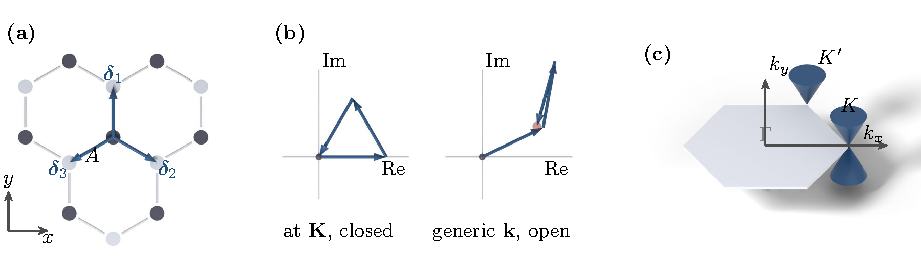
\includegraphics{figures/pdf/s02f04_dirac.pdf}
\end{aqmfigure}
